\section{Setup, and Five Defects in Our Own Harness}
\label{sec:setup}

This section is partly a methods description and partly an audit. The audit
comes first, because eight errors in our own comparison harness and claims
biased the measurements before any architectural conclusion could be drawn,
and five of the eight biased the same way --- against the autoregressive
baseline. We found all eight by re-reading committed artifacts, not by running
new experiments, and the corrections moved headline numbers by more than the
effects we had been reporting. Five are harness defects (items~1--5); three
are claims withdrawn because the measurement behind them was contaminated
(items~6--8), formerly reported in \S\ref{sec:negative}.

\subsection{The stack everything is measured on}

Every measurement from issue \#57 onward runs on a single pinned stack
(Table~\ref{tab:stack}). A shared provenance helper, which no runner can
bypass, writes the model id, revision, runtime versions, GPU, dtype, and every
decoding knob into each result file --- taken from the object that actually
loaded the model, not from a command-line default. A build check
(\artifact{paper/verify\_numbers.py}) fails when a cited artifact lacks that
block. The helper exists because it had to: three result files recorded an
autoregressive model name for diffusion runs (defect 5, below).

\begin{table}[h]
\centering
\caption{The pinned stack. Every number in this paper is measured here unless
explicitly labelled otherwise.}
\label{tab:stack}
\begin{tabular}{@{}ll@{}}
\toprule
\thead{Component} & \thead{Version} \\
\midrule
\tabfont Serving runtime & \tabfont vLLM \vllmVersion~\cite{vllm2023} \\
\tabfont Framework       & \tabfont torch \torchVersion \\
\tabfont Accelerator     & \tabfont \gpuModel \\
\tabfont Precision       & \tabfont BF16 \\
\tabfont Diffusion scheduling & \tabfont serial, \texttt{-{}-max-num-seqs 1} \\
\tabfont Sample size     & \tabfont $n = \nPerCell$ events per cell \\
\bottomrule
\end{tabular}
\end{table}

The serial-diffusion setting is forced, not chosen: vLLM \vllmVersion\ crashes
in \artifact{diffusion\_gemma.py} as soon as two running requests mix
denoising phases. Serialised serving is therefore the diffusion arm's
production-relevant mode on this runtime, and \S\ref{sec:batching} treats that
as the finding it is rather than as an inconvenience.

\subsection{Task and metric}

The task is log-to-record extraction: given one raw log line from
LOGHUB~\cite{loghub} (BGL for the main sweeps, HDFS for the generalisation
check), emit a JSON record. The prompt is a few-shot template of roughly \refPrompt\ tokens.
Quality is macro F1 over fields, and we score \emph{nine} of the twelve
schema fields. The three we drop --- \texttt{event\_type},
\texttt{affected\_entity}, \texttt{remediation\_hint} --- have degenerate gold
labels on BGL: across 2{,}000 events they take 2, 1, and 1 unique values
respectively, so a model that emits an empty object scores $1.000$ on two of
the three by trivially matching a constant. \S\ref{sec:exchange} shows what
that contamination does to the comparison. Both metrics are computed on every
run; only the 9-field number is cited in comparison tables.

\subsection{Numeric precision}

Every number in this paper is quoted to a precision its measurement error
supports. \S\ref{sec:laws} makes that statement for one number --- ``quote it
to one decimal and no further'' --- and this section makes it policy for all of
them, enforced as a lint by \artifact{paper/verify\_numbers.py} over
\artifact{macros.tex}. Latency is quoted to $0.1$\,ms: the run-to-run CV on the
pinned stack is \arCV--\dgCV\%, so $0.1$\,ms is real resolution at the p50 and
anything finer is noise. F1 scores are quoted to three decimals: at
$n = \nPerCell$ events the standard error of a nine-field macro F1 is roughly
$0.006$, so three decimals is the defensible resolution and a fourth is not.
Ratios and multipliers are quoted to one decimal. Fitted coefficients are
quoted only to the precision the residuals support, which is why the K-sweep
decomposition is cited as a shape rather than a measurement: at $R^2 =
\kfitRsq$ its intercept \kfitBase\,ms and slope \kfitSlope\,ms per step are
not interpretable to the precision stated, and we say so wherever they appear.

\subsection{Pricing the Baseline}

\begin{figure}[t]
\centering
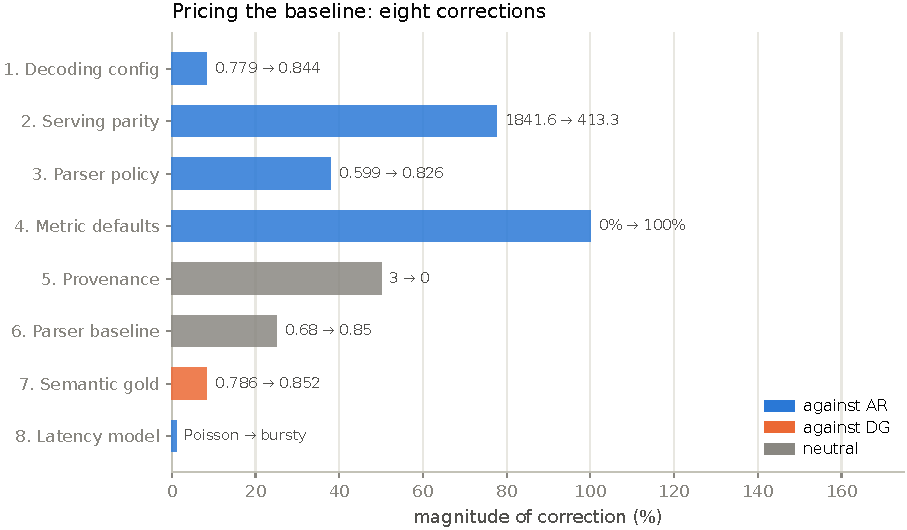
\includegraphics[width=\linewidth]{figures/fig8_defects.pdf}
\caption{Pricing the baseline: eight corrections to our own measurements and
claims. Each row is one item: the value as originally recorded, the value
after the fix, and which arm the bias favoured. Rows~1--5 are harness
defects; rows~6--8 are claims withdrawn because the measurement behind them
was contaminated. Five of the eight biased against the autoregressive arm,
one (row~7) against the diffusion arm, and two were neutral. All eight were
found by re-reading committed artifacts.}
\label{fig:defects}
\end{figure}

\paragraph{1. Decoding configuration}
HuggingFace \texttt{generate()} honours \texttt{repetition\_penalty} even
under \texttt{do\_sample=False}, and Qwen2.5 ships a checkpoint default of
1.1 at 1.5\,B and 1.05 at 3\,B/7\,B. Extraction consists almost entirely of
copying spans out of the input, which is exactly what that penalty suppresses:
it emptied the \texttt{host} field on 80 of 100 events. DiffusionGemma's
hand-written denoising loop has no equivalent default, so the handicap was
one-sided. Setting every knob explicitly on both arms moved \ARoneb\ Field-F1
from \defectOneFBefore\ to \defectOneFAfter.

\paragraph{2. Serving parity}
The autoregressive arm ran a naive HuggingFace generation loop while the
diffusion arm ran a production engine, and the difference was reported as an
architectural result. Putting the autoregressive arm on vLLM moved its p50
from \defectTwoBefore\ to \defectTwoAfter~ms --- \defectTwoRatio$\times$ ---
and reversed the direction of the headline speed claim.

\paragraph{3. Parser policy under over-generation}
When forced to emit $L{=}512$ tokens, \rambleRate\% of autoregressive outputs
contained more than one JSON object: the model finishes the record at its
natural length ($\sim$\naturalLar\ tokens) and then starts another. The old
parser took the span from the first brace to the \emph{last} brace and a
regex fallback assigned fields left-to-right, so the final, most-drifted copy
of each field was the one scored. Re-scoring the \emph{same saved
generations} with first-object-wins moved \ARthree\ at $L{=}512$ from
\defectThreeBefore\ to \defectThreeAfter. DiffusionGemma rambles on 1--3\% of
events and is parser-invariant, so again the defect reached one arm only.
The diagnostic generalises: high schema validity alongside collapsing
per-field accuracy is a parser signature, because a model that is genuinely
degrading loses validity too.

\paragraph{4. Metric behaviour on valid defaults}
The completeness metric compared \texttt{rec.get(f)} against the defaults
\texttt{""}, \texttt{0.0}, and \texttt{False} --- which are structurally valid
values, not missing keys. The autoregressive model stops early and emits falsy
defaults; DiffusionGemma always fills every field. Distinguishing an absent
key from a present-but-falsy one moved \ARthree\ record completeness from
\defectFourBefore\% to \defectFourAfter\%, and \emph{refuted} the finding it
had been supporting.

\paragraph{5. Provenance}
A command-line default survived into three result files, recording an
autoregressive model name for runs of the diffusion model. This biases no
comparison, which makes it the worst of the five in one specific sense: it is
a correctness-of-record defect, and it made audit impossible until correction
sidecars were written.

\paragraph{6. Classical-parser baseline}
An earlier draft claimed a classical parser matched LLM extraction at a
Field-F1 of $0.68$ against $0.85$. What was recorded as a near-match was
self-grading: our ``Drain''~\cite{drain} was a regex fallback rather than the
reference implementation, and the gold generator was the same code, so on
semantic fields the parser was marking its own output. What it should have
been is the gap the comparison actually shows --- the parser is well behind
the LLM, and the claim is withdrawn. The error inflated a third baseline
rather than either architecture, so it is neutral to the AR--DG comparison.
Found by re-reading the gold-generation script.

\paragraph{7. Contaminated semantic gold}
An earlier draft claimed structural and semantic fields separate cleanly. What
was recorded was a 12-field macro on which \ARthree\ leads \DG\ by
\twelveGap\ F1. What it should have been is the decontaminated 9-field macro,
on which the two differ by \qualityGap: the semantic gold labels are
placeholder output of that same parser, and one of them is a constant across
2{,}000 events, so ``semantic F1'' was measuring agreement with a regex. The
contamination inflated the arm that fills fields with plausible text
(\ARthree) and penalised the arm that leaves unpopulated fields empty (\DG),
so this error favoured the autoregressive arm. Found by re-reading the gold
labels.

\paragraph{8. Queueing model for diffusion latency}
An earlier draft claimed an M/D/1 queue predicts diffusion latency under
load. What was recorded was a match to the measured saturation knee under
Poisson arrivals. What it should have been is the same test under bursty
(MMPP) arrivals, which is what log streams actually look like: there the
model stops being predictive. The error overstated how well the diffusion
arm's load behaviour is modelled, favouring the diffusion arm. Found by
re-reading the arrival generator.

\paragraph{The asymmetry is the point}
A comparison harness written by someone hoping the new architecture wins fails
\emph{asymmetrically}. The failures are not random: they cluster on the arm
the experimenter is not rooting for, because that arm inherits the checkpoint
defaults, the naive serving path, and --- ironically --- the mature
production infrastructure that the new architecture is being compared against.
Five of the eight items above biased against the autoregressive baseline; one
(item~7) ran the other way, inflating the autoregressive arm on a
contaminated metric, and two were neutral. The five harness checks in
\artifact{CHECKLIST.md} each take under five minutes, and each catches a
failure that moved a headline number by more than the effect it was
reporting.
